\documentclass{beamer}
\usetheme{Antibes}
\useinnertheme{rectangles}
\useoutertheme{infolines}
\usepackage[utf8]{inputenc}
\usepackage[T1]{fontenc}
\usepackage[ngerman]{babel}

% patch the look of +, = in arev
\usefonttheme{serif} 

\usepackage{arev}
\usepackage{amsmath}
\usepackage{amssymb}

\setbeamertemplate{footline}{%
\begin{beamercolorbox}[ht=3.0ex,dp=1ex]{title in head/foot}
\hfill\footnotesize\insertpagenumber\enspace\enspace\end{beamercolorbox}}

\definecolor{bluegreen1}{rgb}{0.0,0.20,0.28}
\definecolor{bluegreen2}{rgb}{0.0,0.20,0.28}
\setbeamercolor*{palette primary}{fg=white,bg=bluegreen1}
\setbeamercolor*{palette secondary}{fg=white,bg=bluegreen2}
\setbeamercolor*{palette tertiary}{fg=white,bg=bluegreen2}
\setbeamercolor{itemize item}{fg=black}
\setbeamercolor{block title}{bg=bluegreen2}
\newcommand{\modest}[1]{{\small\color{gray}#1}}

\newcommand{\ee}{\mathrm e}
\newcommand{\ui}{\mathrm i}
\newcommand{\real}{\operatorname{Re}}
\newcommand{\imag}{\operatorname{Im}}
\newcommand{\uv}[1]{\underline{#1}}
\newcommand{\bv}[1]{\mathbf{#1}}

\newcommand{\N}{\mathbb N}
\newcommand{\Z}{\mathbb Z}
\newcommand{\Q}{\mathbb Q}
\newcommand{\R}{\mathbb R}
\newcommand{\C}{\mathbb C}

\newcommand{\id}{\operatorname{id}}
\newcommand{\sgn}{\operatorname{sgn}}
\newcommand{\Abb}{\operatorname{Abb}}
\newcommand{\unit}[1]{\mathrm{#1}}
\newcommand{\chem}[1]{\mathrm{#1}}
\newcommand{\strong}[1]{\textsf{\textbf{#1}}}
\newcommand{\defiff}{\quad:\Longleftrightarrow\quad}

\title{Was ist Ableiten?}
\date{}

\begin{document}

\begin{frame}
\maketitle
\end{frame}

\begin{frame}[t]
\vspace{2em}
Gegeben sei eine beliebige reelle Funktion $f$\\
und eine beliebige feste Stelle $x_0$.\pause

\vspace{-1em}
\begin{center}
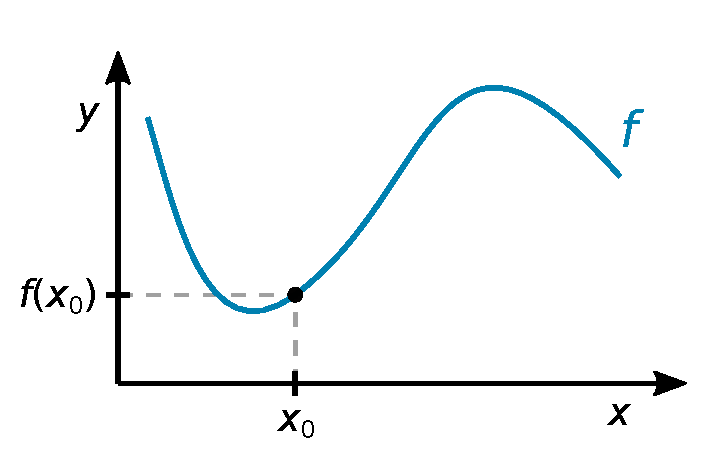
\includegraphics[width=80mm]{img/Funktion.pdf}
\end{center}
\end{frame}

\begin{frame}[t]
\vspace{1em}
Was ist eine reelle Funktion?\pause

\vspace{0.6em}
\strong{Beispiel.} Wir wollen ein
rechteckiges Gartenbeet mit einem festen Umfang $u=4\,\unit{m}$
anlegen. Die Länge des Beetes sei $x$, und die Breite sei $b$.
Der Flächeninhalt des Beetes sei $y$, also gilt $y=x\cdot b$.\pause

\vspace{-1em}
\begin{center}
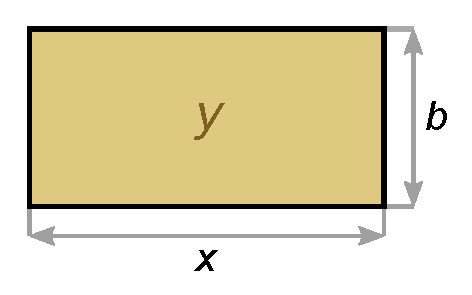
\includegraphics[width=60mm]{img/Beet.pdf}
\end{center}
\end{frame}

\begin{frame}
Außerdem gilt $u=2x+2b$. Umstellen dieser Gleichung nach $b$ bringt
uns $b=\tfrac{u}{2}-x$.\pause{}
Setzen wir dies in die Gleichung $y=xb$ ein,
ist der Flächeninhalt eine Funktion von $x$ gemäß
\[y = f(x),\;\text{wobei}\;\; f(x) := x\cdot (\tfrac{u}{2}-x).\]
\pause
Frage: Wie müsste man $x$ wählen, damit der Flächeninhalt $y$
maximal wird? 
\end{frame}

\begin{frame}[t]
\vspace{1em}

Betrachten wir den Graph am Punkt $(x_0,f(x_0))$ unter einem
genügend starken Mikroskop.\pause

\vspace{0.5em}
$\Longrightarrow$ Bei einer gutartigen Funktion wird der Graph dann
näherungsweise aussehen wie eine Gerade.\pause

\vspace{-1em}
\begin{center}
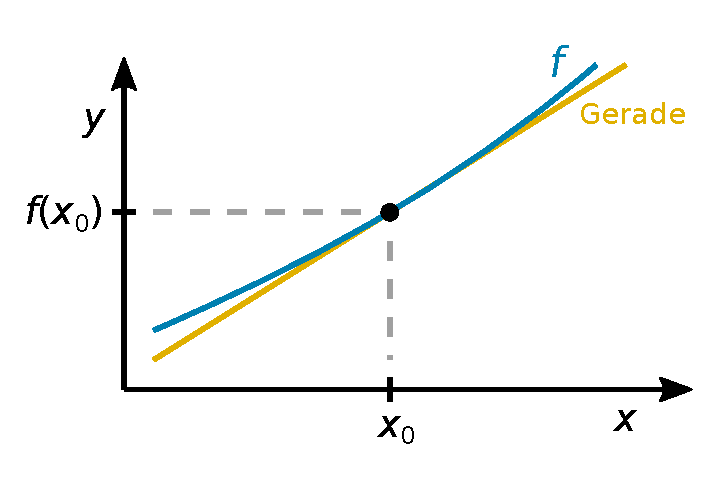
\includegraphics[width=80mm]{img/Funktion-Tangente.pdf}
\end{center}
\end{frame}

\begin{frame}
\strong{Das ist eine wichtige Beobachtung!}\pause

\vspace{0.8em}
Diese Gerade nennen wir \emph{Tangente}.
\end{frame}

\begin{frame}[t]
\vspace{0.5em}
Wir wissen, dass die Tangente durch die Funktion
\[x\mapsto f(x_0)+a\cdot (x-x_0)\]
beschrieben wird, wobei der Anstieg $a$ zunächst\\
unbekannt ist.\pause

\vspace{-1em}
\begin{center}
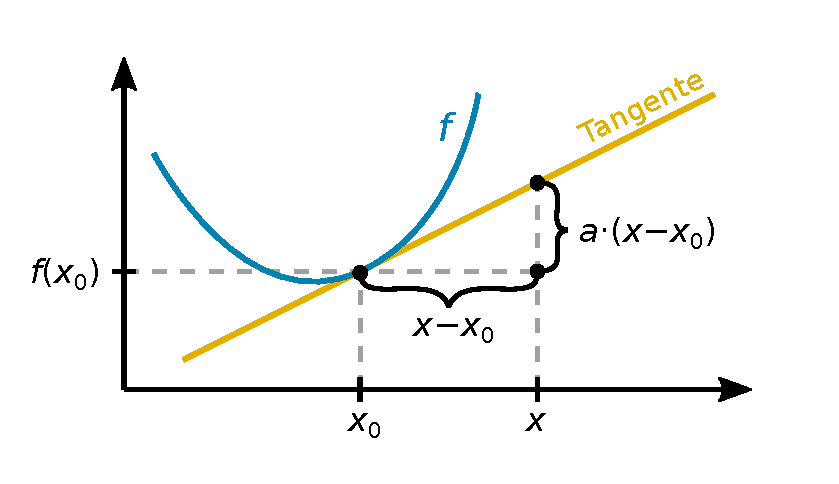
\includegraphics[width=100mm]{img/Tangente.pdf}
\end{center}
\end{frame}

\begin{frame}
\vspace{0.8em}
Für ein $x\approx x_0$ ist also $f(x)\approx f(x_0)+a\cdot (x-x_0)$.
\pause

\vspace{0.8em}
Stellt man diese Gleichung nach $a$ um,\pause{} findet man

\[a \approx \frac{f(x)-f(x_0)}{x-x_0}.\]\pause

Das muss umso genauer werden, je geringer der Abstand zwischen
$x$ und $x_0$ ist.\pause

\vspace{0.8em}
Für $x\to x_0$ kommt da ein ganz bestimmter Anstieg heraus, den
wir \emph{Differentialquotient} nennen. Das ist der
Anstieg der Tangente.
\end{frame}

\begin{frame}
\begin{Definition}
Eine Funktion $f$ heißt \emph{differenzierbar}
an der Stelle $x_0$, wenn der Grenzwert
\[f'(x_0) := \lim_{x\to x_0}\frac{f(x)-f(x_0)}{x-x_0}\]
existiert. Man bezeichnet die Zahl $f'(x_0)$ als \emph{Ableitung} oder
\emph{Differentialquotient} von $f$ an der Stelle $x_0$.
\end{Definition}
\end{frame}

\begin{frame}
Eine Bemerkung dazu. Die Ersetzung $x=x_0+h$ vereinfacht einige
Rechnungen.\pause

\vspace{0.8em}
Man bekommt die äquivalente Formel
\[f'(x_0) := \lim_{h\to 0} \frac{f(x_0+h)-f(x_0)}{h}.\]
\end{frame}

\begin{frame}
Die Bestimmung von Ableitungen ist recht einfach, weil man dafür
\emph{Ableitungsregeln} herleiten kann, die das auf die Terme
zurückführen, aus denen der gegebene Funktionsterm
zusammengesetzt ist.\pause

\vspace{0.8em}
Außerdem lässt sich die Ableitung näherungsweise auch ganz leicht
numerisch berechnen. Man setzt z.\,B. für $h$ einfach eine sehr
kleine Zahl ein.
\end{frame}

\begin{frame}
Ja, gut. Aber wozu soll das denn nützlich sein?
\end{frame}

\begin{frame}
Eine der wichtigsten Anwendungen sind Extremwert-Aufgaben.\pause

\vspace{0.8em}
Hierbei ist $f(x)$ eine Größe in Abhängigkeit von $x$, die
man maximieren oder minimieren möchte.
\end{frame}

\begin{frame}[t]
\vspace{1em}
Grundlegende Beobachtung: Hat eine differenzierbare Funktion $f$ an
einer Stelle $x$ ein Extremum, dann muss dort eine waagerechte
Tangente vorliegen.
\pause

\vspace{-1em}
\begin{center}
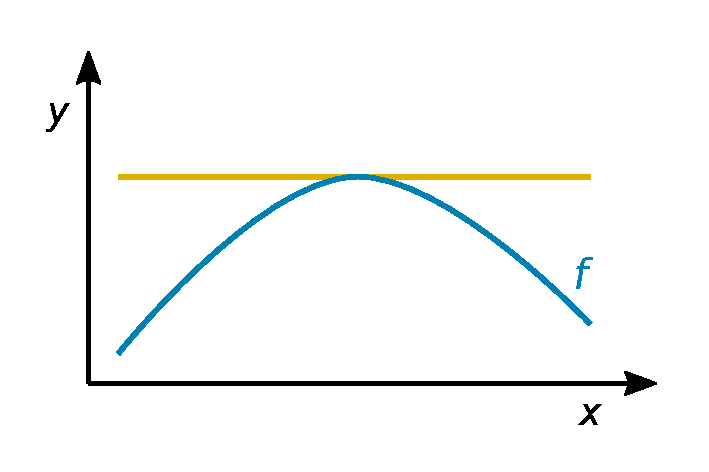
\includegraphics[width=80mm]{img/Maximum.pdf}
\end{center}
\end{frame}

\begin{frame}
Ergo: Bei einer Extremstelle muss $f'(x)=0$ sein.
\pause

\vspace{0.8em}
Umgekehrt können wir nun durch Lösen der Gleichung $f'(x)=0$ nach
solchen Stellen fischen. Zwar müssen nicht alle Lösungen auch
Extremstellen sein, aber es kann keine Extremstelle geben, die nicht
Lösung dieser Gleichung ist. {\footnotesize
(Ausgenommen davon sind die Randstellen des Definitionsbereichs.)}
\pause

\vspace{0.8em}
Man nennt $f'(x)=0$ ein \emph{notwendiges Kriterium} für eine
Extremstelle.
\end{frame}

\begin{frame}
Zurück zum Beet.\pause{} Hier rechnet man
\begin{align*}f(x+h) &= (x+h)\cdot(\tfrac{u}{2}-(x+h)) = (x+h)\cdot(\tfrac{u}{2}-x-h)\\
&= \underbrace{x\cdot(\tfrac{u}{2}-x)}_{f(x)} + h\cdot (\tfrac{u}{2}-x) - xh - h^2.
\end{align*}\pause
Somit gilt
\[\frac{f(x+h)-f(x)}{h} = (\tfrac{u}{2}-x) - x - h = \tfrac{u}{2}-2x-h.
\]\pause
Für $h\to 0$ ergibt sich schließlich $f'(x) = \tfrac{u}{2}-2x$.
\end{frame}

\begin{frame}
Die notwendige Bedingung $0=f'(x)=\tfrac{u}{2}-2x$ formen wir nach
$x$ um.\pause

\vspace{0.8em}
Das bringt $x = \tfrac{u}{4} = \tfrac{4\,\unit{m}}{4} = 1\,\unit{m}$.
\pause

\vspace{0.8em}
Fazit: Nur die Länge $x = 1\,\unit{m}$ führt zum maximalen
Flächeninhalt, sofern es überhaupt einen solchen gibt.

\vspace{0.8em}
Das ist ein quadratisches Beet.
\end{frame}

\begin{frame}
\begin{center}
\strong{Höhere Mathematik}
\end{center}
\end{frame}

\begin{frame}
Angenommen, $f$ ist von mehreren Variablen abhängig. Wir würden
auch gerne Extremstellen einer solchen Funktion ermitteln.
\end{frame}

\begin{frame}
Fasse die Variablen zu einem Vektor
$\mathbf x:=(x_1,\ldots,x_n)$
zusammen.\pause

\vspace{0.8em}
Man betrachte an einer Stelle $\mathbf x$ nun einen Verschiebungsvektor
$\mathbf v$, der $\mathbf x$ an eine andere Stelle im selben
Definitionsbereich verschiebt. Skaliert man $\mathbf v$ vorher
mit der Zahl $t$, wird die Verschiebung beschrieben durch den Term
$\mathbf x+t\mathbf v$. Die Funktion
$g(t):=f(\mathbf x+t\mathbf v)$ ist wieder
eine gewöhnliche reelle Funktion, von welcher wir ja die Ableitung
$g'(0)$ bestimmen können. Diese nennt man \emph{Richtungsableitung}
von $f$ in Richtung $\mathbf v$ an der Stelle $\mathbf x$.
\end{frame}

\begin{frame}[t]
\vspace{2em}
Für die Anschauung betrachten wir immer den Fall
$\mathbf x = (x_1,x_2)$.
\pause

\vspace{-1em}
\begin{center}
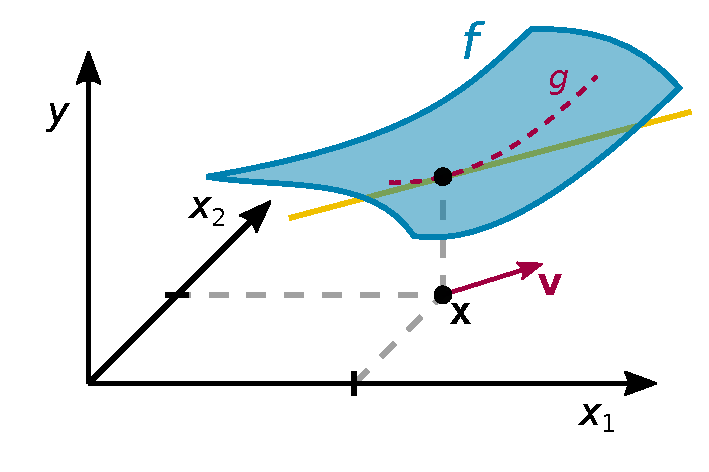
\includegraphics[width=80mm]{img/Richtungsableitung.pdf}
\end{center}
\end{frame}

\begin{frame}
\begin{Definition}
Die Richtungsableitung von $f$ an der Stelle $\mathbf x$ in
Richtung $\mathbf v$ ist definiert als der Grenzwert
\[D_{\mathbf v} f(\mathbf x) := \lim_{h\to 0}\frac{f(\mathbf x+h\mathbf v)-f(\mathbf x)}{h}.\]
\end{Definition}
\end{frame}

\begin{frame}[t]
\vspace{1em}
Beobachtung: Bei einer Extremstelle liegt eine waagerechte
Tangentialebene vor. D.\,h. es muss $D_{\mathbf v} f(\mathbf x)=0$
sein, und das in jede Richtung $\mathbf v$.\pause

\begin{center}
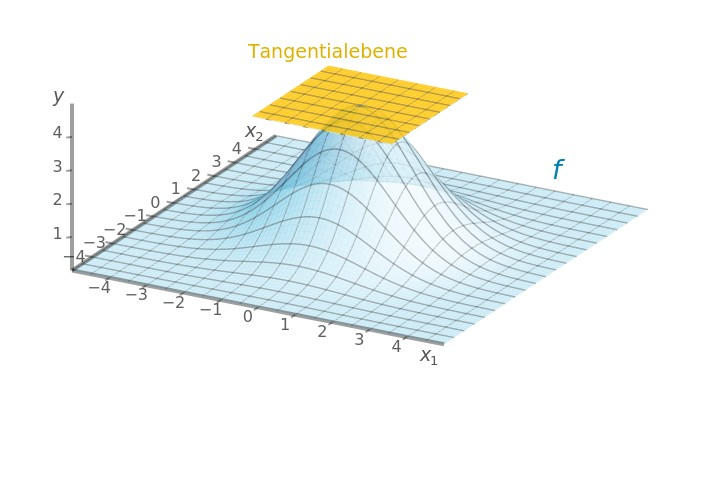
\includegraphics[width=100mm]{img/Maximum2.jpg}
\end{center}
\end{frame}

\begin{frame}
Das ist eine Verallgemeinerung des notwendigen Kriteriums.
\pause

\vspace{0.8em}
Bemerkung: Speziell für $\mathbf v = \mathbf e_k$, wobei
$\mathbf e_k$ der Einheitsvektor in Richtung der $k$-ten Achse ist,
spricht man von der \emph{partiellen Ableitung}
$\partial_k f(\mathbf x)$.
\pause

\vspace{0.8em}
Bei einer gutartigen Funktion $f$ genügt
$\partial_k f(\mathbf x)=0$ für alle $k$, dann ist bereits
$D_{\mathbf v}f(\mathbf x)=0$ für alle $\mathbf v$.
\end{frame}

\begin{frame}
Die partiellen Ableitungen fasst man zu einem (Ko)Vektor zusammen,
der \emph{totales Differential} genannt wird.\pause

\begin{Definition}
Totales Differential von $f$ an der Stelle $\mathbf x$:
\[\mathrm df(\mathbf x) := \sum_{k=1}^n \partial_k f(\mathbf x)\,\mathrm dx_k.\]
\end{Definition}
\pause

Das notwendige Kriterium lautet dann kurz: $\mathrm df(\mathbf x)=0$.
\end{frame}

\begin{frame}
\begin{footnotesize}
Bemerkung: Das totale Differential kodiert die Information über den
Anstieg in die unterschiedlichen Richtungen. Die partielle
Ableitung $\partial_k f$ ist gerade der Anstieg in Richtung der
$k$-ten Achse.
\end{footnotesize}
\end{frame}

\begin{frame}
\begin{center}
\strong{Noch höhere Mathematik}
\end{center}
\end{frame}

\begin{frame}
Bei der Richtungsableitung kann man auf die Idee kommen, für
$\mathbf x$ und $\mathbf v$ Funktionen einzusetzen.
\pause

\vspace{0.6em}
Warum das?
\pause

\vspace{0.6em}
Im Ausdruck $\mathbf x+h\mathbf v$ kommt lediglich eine
Multiplikation mit dem Skalar $h$ und eine vektorielle Addition vor.
Das klappt in allen Vektorräumen, und damit auch in Funktionenräumen.
\pause

\vspace{0.8em}
Diese Verallgemeinerung der Richtungsableitung wird
\emph{funktionale Ableitung} genannt. -- Unter zusätzlichen
Prämissen spricht man von der \emph{Gâteaux-Ableitung}.
\end{frame}

\begin{frame}
Was ist ein Funktionenraum?\pause

\vspace{0.8em}
Betrachte einen Vektorraum $Y$
und einen beliebigen Definitionsbereich $X$. Dann sind
Funktionen $f,g\colon X\to Y$ als Vektoren zu verstehen, indem
man die Multiplikation mit dem Skalar $h$ und
die Addition so definiert:
\begin{align*}
& (hf)(t) := hf(t),\\
& (f+g)(t) := f(t)+g(t).
\end{align*}
\end{frame}

\begin{frame}
\begin{Definition}
Sei $V$ ein Vektorraum und $F$ ein Funktional, d.\,h. $F\colon V\to\R$.

\vspace{0.6em}
Funktionale Ableitung von $F$ an der Stelle $x$ in Richtung $v$:
\[\delta_v F(x) := \lim_{h\to 0}\frac{F(x+hv)-F(x)}{h}.\]
\end{Definition}\pause

Bemerkung: Die Größe $hv$ nennt man \emph{Variation} von $x$.
\end{frame}

\begin{frame}
Bei der Extremwert-Aufgabe muss wieder $\delta_v F(x)=0$ für alle
$v$ sein.
\pause

\vspace{0.8em}
Das führt nun allerdings zu einem frappierenden Rechenwerkzeug,
der \emph{Variationsrechnung}.
\end{frame}

\begin{frame}
Für das als bestimmtes Integral* formulierte Funktional
\[F(x) := \int_a^b L(t,x(t),x'(t))\,\mathrm dt\]
führt die Extremwert-Aufgabe -- d.\,h. die Suche nach einem Extremwert
von $F$ -- zur Euler-Lagrange-Gleichung der Variationsrechnung.
\end{frame}

\begin{frame}

{\footnotesize
*Das bestimmte Integral $\int_a^b f(t)\,\mathrm dt$
ist (für $f(t)\ge 0$) der Flächeninhalt unter dem Graph
von $f$ für $a\le t\le b$.}
\begin{center}
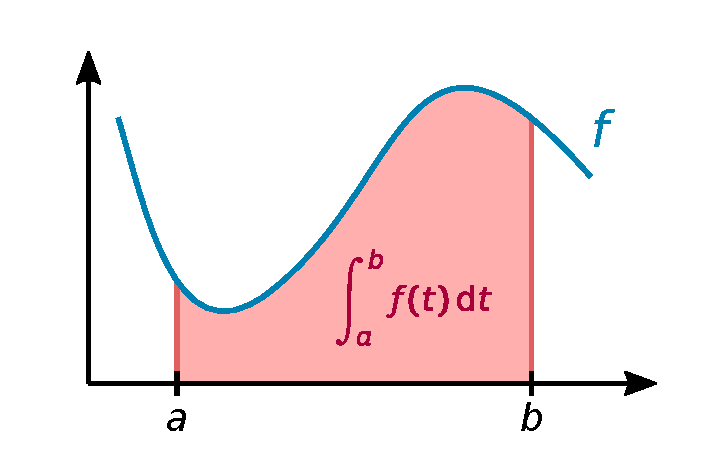
\includegraphics[width=80mm]{img/Integral.pdf}
\end{center}
\end{frame}

\begin{frame}
Wozu braucht man das?\pause

\vspace{0.8em}
Die Variationsrechnung hat sich als fundamentales Werkzeug der Physik
erwiesen. Im 20. Jhd. gewann man damit einen äußerst tief liegenden
Einblick in die Beschaffenheit des Kosmos.
\end{frame}

\begin{frame}
Anwendungen der Variationsrechnung:
\begin{itemize}
\item Der Lagrange-Formalismus, Grundstein der analytischen Mechanik.

\item Damit auch Verständnis des Noether-Theorems, einem
Fundamentalsatz der Physik, der Symmetrien und Erhaltungsgrößen
in Beziehung setzt.

\item Herleitung der Grundgleichungen von klassischen Feldtheorien,
z.\,B. die Maxwell-Gleichungen.

\item Herleitung der Feldgleichungen der allgemeinen
Relativitätstheorie (Einstein-Hilbert-Wirkung).

\item Maßgebliches Werkzeug der Quantenfeldtheorien.
\end{itemize}
\end{frame}

\begin{frame}
Ende.
\vfill\hfill\modest{Juli 2020}\\
\hfill\modest{Creative Commons CC0}
\end{frame}


\end{document}


